\chapter{Sensitivity Studies for G3 Dark Matter}
\label{chap:chap6}

Second generation dual-phase liquid xenon detectors due to go online, such as LZ and XENONnT, are projected to reach SI-WIMP sensitivities of $\sim1.4 \times 10^{-48}$ cm$^{2}$ at a 90\% CL \cite{akerib2018projected, xenon_1t}. In comparison to their predecessors, they will probe the WIMP dark matter paradigm with orders of magnitude improvement. However, a significant amount of the parameter space prior to the cosmic neutrino background---the so called \textit{neutrino floor}---will remain to be explored. In an effort to examine the necessary scale of a future LXe detector and the required background levels to probe down to the neutrino floor, a third-generation (G3) toy LXe detector was envisioned. This chapter outlines the rationale behind a G3 experiment and the assumptions made in constructing a potential sensitivity curve for the SI WIMP paradigm by using LZ as a model detector and the \textsc{LZStats} package to assess the statistical reach. 


%%------------------------------$$
\section{Motivation}
\label{sec:motivation}
%%------------------------------$$

The primary purpose of a third-generation (G3) dark matter experiment using dual-phase xenon technology will be focused towards designing a detector with optimal sensitivity for WIMPs. Furthermore, with the scale of a G3 experiment, there is a real possibility of transitioning from an experiment focusing mainly on WIMP dark matter, to one which operates as an observatory for a range of rare event physics searches. Some of these avenues include the search for neutrinoless double beta decay with pre-existing isotopes of \XeOTF{} and \XeOTS{}, and the study of solar and cosmic neutrinos, provided enough active LXe is present. The current generation experiments, such as LZ and XENONnT, are soon to begin data taking, with sensitivity projections for the SI WIMP-nucleon interaction around $\sim1.4 \times 10^{-48}$ cm$^{2}$ for a 40 GeV/c$^{2}$ mass WIMP at a 90\% CL \cite{akerib2018projected, Aprile:2020vtw}. Although these experiments are expected to probe a considerable magnitude of the favoured phenomenological MSSM parameter space \cite{pMSSM11}, their reach is restricted by various backgrounds and the scale of the active LXe mass. However, a significant amount of the pMSSM parameter space prior to the cosmic neutrino background---which poses a hard boundary on the WIMP discovery potential---will remain to be explored. Exploring cross-sections below $\sim10^{-49}$ cm$^{2}$ is extremely difficult given the uncertainties on the neutrino fluxes and their irreducible nature in the $S1\mhyphen{}S2$ space; thus, precise measurements of different neutrino flux components are of utmost importance for a G3 experiment and beyond in reducing the impact of neutrino backgrounds on direct detection experiments \cite{neutrino_floor}.

There are several sources of known background events expected in a potential G3 detector, similar to those expected in G2 experiments, as detailed in chapters \ref{chap:chap4} \& \ref{chap:chap5}. The degree in which these backgrounds impact the potentiality of a discovery varies with the search type and therefore the energy scale of the search region of interest. Despite their production mechanisms, these backgrounds are observed either as NRs or ERs for the WIMP hypothesis, and hence are more or less WIMP-like, respectively. Isotopic backgrounds originating from material and components, surface contamination and the environment are all expected to contribute to the overall background rates. Therefore, beyond the scaling of the detector, a G3 experiment will require similar or improved techniques of screening, handling and construction of the detector to reduce background rates. The rates expected from the material specific backgrounds depend on various factors: location of experiment, material selection and cleanliness, veto detector efficiency, xenon purification efforts and other variables; hence their rates can be altered and reduced through a multitude of approaches.

A major background contribution to the WIMP search ROI is from astrophysical neutrinos. The elastic neutrino-electron scattering \cite{HASERT1973138} and coherent elastic neutrino-nucleus scattering (CE$\nu$NS) \cite{Akimov_2017} lead directly to ER and NR events, respectively. There are several sources of neutrino backgrounds observable more prominently by a future G3 detector; atmospheric neutrinos produced in muon and pion decays, neutrinos produced in distant supernovae events, and solar neutrinos originating from various fusion reactions within the sun. The solar neutrino background for WIMP masses greater than $\sim$20GeV/c$^{2}$ is dominated by \textit{pp} neutrinos, with contributions from the \BeS{} and CNO (Carbon-Nitrogen-Oxygen) cycles, and are expected to become the largest ER contribution at G3 scales. The \BE{} and \textit{hep} neutrino rates significant for NR energies $\lesssim 6$ keV---equivalent to WIMP masses below $\sim20$ GeV/c$^{2}$---is expected to be observed in $\mathcal{O}(100)$ events. The astrophysical neutrino background rates are independent of detector dependent approaches and hence are irreducible in nature and is expected to be the dominant source of background events for a future G3 experiment in both the ER and the NR bands. Although these signatures are backgrounds to the WIMP analysis, extensive studies on these signatures in theory can lead to improvements for the WIMP search and neutrino physics in general. Albeit, the primary focus of the study highlighted in this chapter is to consider the rates of these backgrounds as inputs into a potential G3 experiment in search for WIMP dark matter to determine the potential parameter space such an experiment can cover. The following sections will detail any potential improvements a G3 experiment can benefit from, the assumptions made in constructing the statistical models, and the results of such an experiment for the SI WIMP sensitivity. 


%%------------------------------$$
\section{Potential Improvements}
\label{sec:g3_improvements}
%%------------------------------$$

A combination of cleanliness protocols and an ultra-selective screening campaign, likes of which has been demonstrated by the LZ collaboration \cite{lz_screening}, is expected to lead to substantial reductions on backgrounds from detector related radioactive isotopes. Moreover, a G3 experiment utilising an outer detector (OD) with a gadolinium load liquid scintillator (GdLS), and a LXe skin veto system with a more stringent fiducial volume that makes use of the self-shielding effect of LXe, is likely to benefit from a significant reduction in detector related backgrounds in comparison to G2 experiments. Furthermore, with more effective shielding---either by utilising a larger water tank or making use of lead-like shielding---a significant reduction on environmental backgrounds may also be expected. Improvements on dispersed xenon contaminants are more challenging in nature. The background rate from the $2\nu\beta\beta$ of \XeOTS{} is expected to be constant, unless isotopic purification of xenon is considered. Current experiments are making use of custom-made gas chromatography systems to expel the \KrEF{}, and in theory can achieve \KrEF{} concentrations of 0.015 ppt \cite{lz_tdr}. The krypton rate is already deemed to be highly ambitious, hence a significant improvement will be highly unlikely for a G3 experiment using tens of tonnes of LXe. 

Without further development, the background from radon emanation, more specifically, the \textit{naked}-\beta{} emission from \PbTOF{} in the \RnTTT{} sub-chain---the current most dominant background in G2 experiments---is expected to be a significant limiting factor in the science reach of a future G3 experiment. With a radon screening campaign selecting low-emanation material and a radon removal system deployed for the gas-phase of the detector \cite{lz_screening, lz_tdr}, the LZ collaboration is projected to achieve a radon activity between 1.10--2.16 $\micro{}$Bq/kg of xenon. Despite these efforts, the background contributions from radon are expected to make up $\sim70\%$ of all ER backgrounds for the WIMP search in LZ \cite{akerib2018projected}. Accurate radon-induced background estimates and characterisation of their impact is challenged by poor understanding of material- and temperature-dependent radon diffusion coefficients and emanation rates. While radon diffusion is suppressed in some material at cryogenic temperatures, radon progeny recoiling out from surfaces is not. There is limited data available on the overall temperature dependence of radon outgassing from material, with even less distinguishing surface from bulk emission. Similarly, there is very limited data on potential radon barriers that could be applied to material surfaces to inhibit radon emanation. A future G3 experiment adopting more accurate radon screening methods, discussed in detail in chapter \ref{chap:chap7}---aimed towards a better understanding of emanation out of varying detector material at LXe temperatures---can lower contributions through a more selective material sourcing process. In addition, the use of potential radon barriers applied on material surfaces can further reduce emanation out of surfaces. Combining these approaches with online radon removal techniques, as demonstrated in \cite{Aprile:2017kop} by the use of cryogenic distillation and analytically-driven approaches in tagging and vetoing the \textit{naked}-\beta{} emission from \PbTOF{}, a substantial reduction in radon-related backgrounds is possible. With a more driven campaign, G3 experiments will likely reduce the impact of radon backgrounds on the WIMP ROI, which will also positively impact any other physics searches in the ER band.  


%%------------------------------$$
\section{Toy G3 Detector \& Background Assumptions}
\label{sec:g3_assumptions}
%%------------------------------$$

In an effort to examine what it takes to probe the remaining parameter space of the pMSSM model and exploiting the full discovery potential of dual-phase xenon TPC technology down to the so-called \textit{neutrino floor}, a toy G3 detector was envisioned. To reach a cross-sectional sensitivity of $\sim10^{-49}$ cm$^{2}$, a future detector would vaguely require a target mass 10 times that of current-generation detectors. The proposed toy detector is conceptualized to be similar to current G2 experiments for simplicity, with a diameter and an active length of 3.14 m, holding a total of 70 tonnes of LXe with the TPC. To reduce detector and wall related backgrounds, a virtual fiducial volume is assumed, cutting away 7.85 cm of active volume from the walls, below the cathode and above the gate, resulting in a fiducial volume of 60 tonnes. A TPC of this size is roughly twice as large as the current-generation detectors and offers a factor of $\sim10$ increase in active mass. In assuming a similar design to its predecessors, its likely that a significant fraction of detector related backgrounds will originate from the top and bottom PMT arrays; which will require around 2300 3-inch-diameter PMTs to provide a similar coverage density as utilised in G2 detectors. 

The detector parameters of a G3 experiment will play a big role in the expected signal and background rates as seen through the reconstructed observables \textit{S1, S2, x-y-z, t}. These variables are fundamentally dependent on the photon detection techniques used in such detectors. A future G3 experiment will likely use a similar approach to G2 experiments in optimising for light and charge collection, through the use of PMTs or silicon photomultipliers \cite{Gundacker_2020} and PTFE coverings to reduce absorption. The end result of such techniques will result in a $g_{1}$, $g_{1gas}$ and a $g_{2}$ factor as described in section \ref{secsec:detector_param}. Although photon and charge collection efficiencies may improve as a result of technological advancements, as a conservative measure, the toy detector assumes identical parameters to that of the LZ experiment, where $g_{1}$ = 0.119 phd/ph, $g_{1gas}$ = 0.102 phd/ph and $g_{2}$ = 79.2 phd/e, as detailed in table \ref{tab:lz_parameters}. These factors are used in converting the scaled background spectra from figures \ref{fig:lz_nr_spectrum} \& \ref{fig:lz_er_spectrum} to the $S1\mhyphen{}S2$ representation needed to construct the background specific PDFs. 


In calculating the sensitivity of a G3 detector to SI WIMPs, a total of 5 live years was assumed, equating to an exposure of 300 tonne$\cdot$years. An 11-component background model including those detailed in sections \ref{secsec:background_table} \& \ref{secsec:plr_input} with projections of improvements for several of the sources are assumed. A simplified background table using a cut-and-count analysis, approximating the number of background counts from a region of interest relevant to a 40 GeV/c$^{2}$ WIMP, approximately 1.5--6.5 keV for ERs and 6--30 keV for NRs, is provided in table \ref{tab:g3_background_count}. The rates of detector related backgrounds and dispersed backgrounds from \RnTTT{} and \RnTTZ{} were scaled by a factor of 0.1 in comparison to LZ. The remaining background contributors were kept at the same rate as LZ for the reasons given in section \ref{sec:g3_improvements}. With these assumed improvements, detector and dispersed radioisotopic backgrounds become sub-dominant to solar backgrounds for ER events. The largest impact to WIMP sensitivity above $\sim20$ GeV/c$^{2}$ is expected to come from atmospheric and solar (\textit{pp} + \BeS{} + \NOT{}) neutrino backgrounds. At energies below 6 keV the solar neutrinos from (\BE{} $+$ \textit{hep}) is dominant. 

Furthermore, topologically non-standard backgrounds that are potentially dangerous for the WIMP search are considered. One of these is accidental coincidence events from PMT dark count and S2-only interactions. Dark count events can lead to fake S1-only events, and very low energy events can show up as S2-only without an S1 component; the combination of which can create an S1-S2 pair in the WIMP ROI. This background component can be estimated using the cold PMT dark count measurement of 25 Hz (reported in \cite{Aprile_2017}) and a 1 mHz S2-only rate (twice that seen in LUX \cite{Akerib_2016}). Taking into account the increased number of PMTs and live days for the proposed toy G3 experiment, the expected coincidental background when enforcing a 3-fold PMT coincidence level is expected to total 29.8 events. This is substantially more significant than that expected in LZ (less than 0.2 events). Increasing the PMT coincidence threshold to 4-fold will reduce the events to less than 0.05 events but this comes at the cost of increasing the low-energy threshold of the detector, thus reducing the sensitivity to lower mass WIMPs. A possible G3 experiment will require more stringent PMT dark count and S2-only rates to sustain a 3-fold coincidence level. 

%
\begin{table}[]
\centering
\caption{Estimated background rates from all significant contributors in a 5 live year run and a 60 tonne fiducial mass. The ER and NR counts are from a region of interest relevant to a 40 GeV/c\squared{} WIMP; approximately 1.5--6.5 keV for ERs and 6--30 keV for NRs; and after application of the single scatter, skin and OD veto cuts. Counts from the solar \BE{} and hep neutrinos are given as a reference, as they are not significant above an NR energy of 6 keV. The ER discrimination of 99.9\% is aimed at selecting ER events from the energy-space that is most relevant for NR interactions.}
\label{tab:g3_background_count}
\vspace{1mm}
\renewcommand{\arraystretch}{1.2}
    \begin{tabularx}{1.0\linewidth}{@{\extracolsep{\fill}}lll}
    \toprule
    \textbf{Background Sources} & %1
    \textbf{ER} & %2
    \textbf{NR} & %3
    \hline
    \hline

    Detector (Det. + Lab. + Cosmo. + Surf.)     & 106  & 1.00 \\
    \textbf{Dispersed radioisotopes (Xenon)}    &      &      \\
    \RnTTT{} (0.18 \micro{}Bq/kg)                & 1333 & 0    \\
    \RnTTZ{} ($9\times10^{-3}$ \micro{}Bq/kg)               & 217  & 0    \\
    \XeOTS{} ($2\nu\beta\beta$)                 & 1311 & 0    \\
    \KrEF{} (0.015 ppt g/g)                     & 528  & 0    \\
    \textbf{Astrophysical neutrinos}            &      &      \\
    Atmospheric (Atm)                           & 0    & 10.4 \\
    Diffuse supernova (DSN)                     & 0    & 1.00 \\
    Solar (\BE{} + \textit{hep})                & 0    & 722* \\
    Solar (\textit{pp} + \BeS{} + \NOT{})       & 4990 & 0    \\
    \hline
    Total                                                       & 8485 & 12.4 \\
    Total (with 99.9\% ER discrimination, 40\% NR efficiency)   & 8.49 & 4.96 \\
    
    \bottomrule
    \end{tabularx}
\end{table}
%

%%------------------------------$$
\section{G3 SI WIMP Sensitivity}
\label{sec:g3_sensitivity}
%%------------------------------$$


The component specific background spectra for the LZ WIMP search analysis, as shown in figures \ref{fig:lz_nr_spectrum} \& \ref{fig:lz_er_spectrum} was scaled and used to produce two dimensional probability density functions (PDFs) using NEST v.2.0.0 in $S1\mhyphen{}S2$ space and fed into a profile likelihood ratio analysis framework used by LZ. The WIMP ROI for this analysis was defined by 0 $<$ S1$_{c}$ $<$ 80 phd, with a 3-fold S1 coincidence requirement. The 3-fold cut is required to reduce background events leaking into the WIMP ROI from coincidences between PMT dark noise and S2-only events---although this background topology still contributes significantly with generation 2 rates for PMT dark noise and S2-only rates, it has been ignored for this study with an anticipation of improvements for a possible G3 experiment. In addition, the S2-raw signal is selected to be greater than 420 phd---equivalent to $\sim5$ extracted electrons. Furthermore, only single scatter events, passing the skin and the OD vetoing were selected and scaled. 

The SI WIMP sensitivity of the toy G3 experiment is evaluated using the same PLR method as described in section \ref{sec:lz_stats}, with an unbinned and extended likelihood, as shown in equation \ref{eq:full_lz_likelihood}, providing optimal exploration between the signal and background models, based on 2-dimensional $S1\mhyphen{}S2$ PDFs. A scan over the parameter of interest, $\mu_{s}$---equivalent to the SI WIMP cross section---at a 90\% confidence level was evaluated for WIMP masses ranging from 5 GeV/c$^{2}$ up to 20,000 GeV/c$^{2}$ by performing a frequentest hypothesis test inversion using the RooStats package \cite{moneta2010roostats}. The sensitivity projection uses a one-sided PLR test statistic in evaluating the upper limit. 

The projected sensitivity for the toy G3 detector with the assumed background scaling and an exposure of 300 tonne$\cdot$years to SI WIMP-nucleon scattering is shown in figure \ref{Fig:si_wimp_sensitivity}. The best sensitivity is achieved at a WIMP mass of 40 GeV/c$^{2}$ with a cross section of $1.2 \times 10^{-49}$ cm$^{2}$. With this sensitivity, the remaining parameter space that G2 experiments will fail to examine above the coherent scattering of neutrinos from astrophysical sources is comfortably reached. For comparison, figure \ref{Fig:si_wimp_sensitivity} also shows the limits achieved by some of the leading dark matter experiment, and those that are projected by current G2 experiments approaching data-taking. Neutrino iso-event contour lines derived for a background-free LXe detector with sub-keV energy threshold from \cite{neutrino_floor} are also presented. The significant reduction in sensitivity observed below 20 GeV/c$^{2}$ WIMP masses is due to the dominance of the solar neutrinos NR background from \BE{} and \textit{hep} neutrinos. 


\begin{figure}[h!]
    \centerline{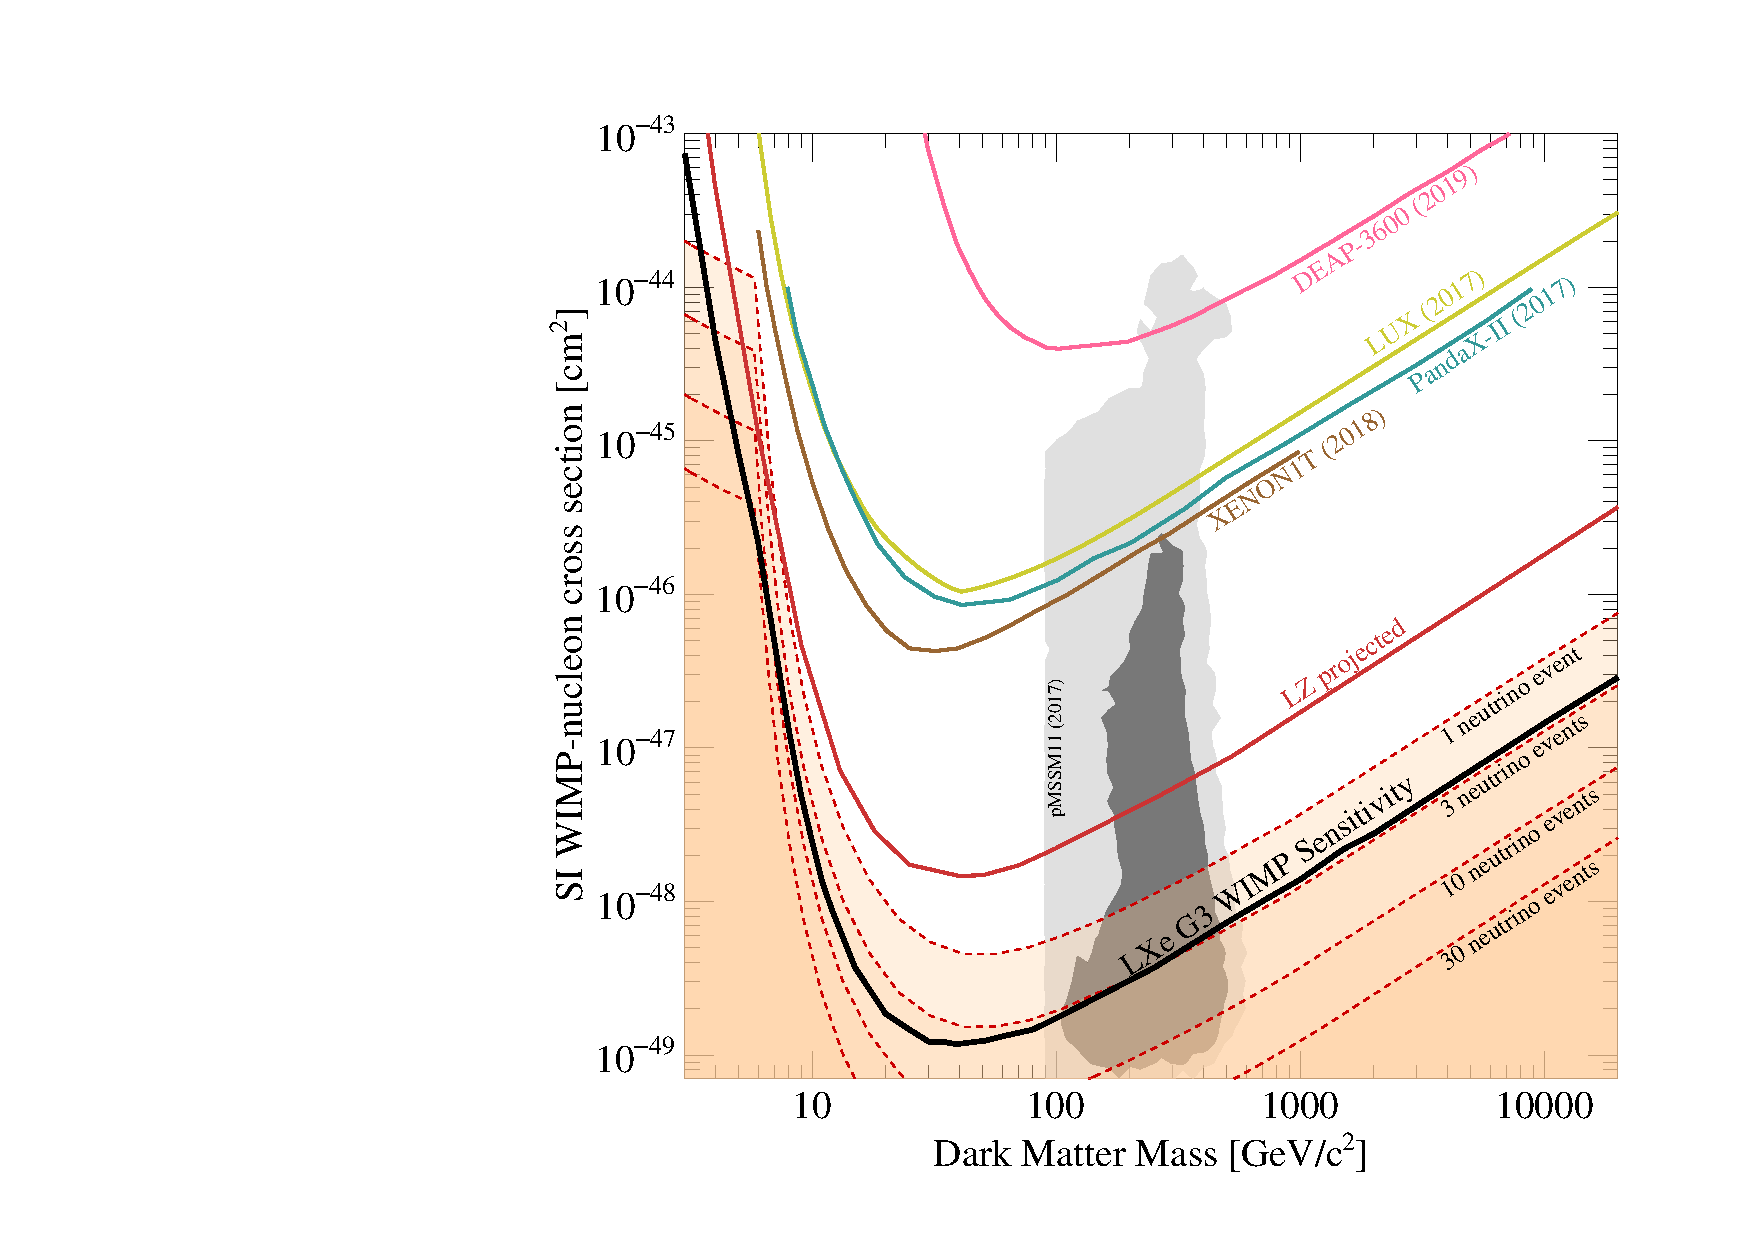
\includegraphics[width=\linewidth]{Chapter_6/Figures/g3dm_si_vs_mass.pdf}}
    \caption
    [Projected sensitivity (90\% CL) to SI WIMP-nucleon elastic scattering for a total exposure of 300 tonne-years.]
    {Projected sensitivity (90\% CL) to SI WIMP-nucleon elastic scattering for a total exposure of 300 tonne-years. A minimum of $1.2 \times 10^{-49}$ cm$^{2}$ is expected at 40 GeV/c$^{2}$. Sensitivity projections from the LZ experiment \cite{akerib2018projected} and exclusion limits achieved by XENON1T \cite{xenon_1t}, PandaX-II \cite{pandax_limit}, LUX \cite{Akerib:2017kat} and the DEAP-3600 \cite{DEAP_3600} collaborations are also provided as a reference. Neutrino isoevent contour lines derived for a background-free LXe detector with sub-keV energy threshold is detailed in \cite{neutrino_floor}.}
    \label{Fig:si_wimp_sensitivity}
\end{figure}

\newpage